\documentclass[titlepage]{article}
\title{Systemd for Administrators}
\usepackage[english]{babel}
\usepackage{hyperref}
\usepackage{graphicx}
\usepackage{listings}
\author{
    Lennart Poettering\\
    \texttt{Author}
    \and
    Christian Rebischke\\
    \texttt{Editor}
}
\lstset{
    basicstyle=\tiny,
    frame=single
}
\setlength{\parindent}{0pt}
\begin{document}
\maketitle
\tableofcontents
\newpage

\section{Abstract}
As many of you know,
\href{https://www.freedesktop.org/wiki/Software/systemd}{systemd} is the new
Fedora init system, starting with F14, and it is also on its way to being
adopted in a number of other distributions as well (for example,
\href{https://en.opensuse.org/SDB:Systemd}{OpenSUSE}). For administrators
systemd provides a variety of new features and changes and enhances the
administrative process substantially. This blog story is the first part of a
series of articles I plan to post roughly every week for the next months. In
every post I will try to explain one new feature of systemd. Many of these
features are small and simple, so these stories should be interesting to a
broader audience. However, from time to time we'll dive a little bit deeper
into the great new features systemd provides you with.  
\section{Disclaimer}
This handbook is written by Lennart Poettering. There are maybe some 
additions, cuts or other changes for increasing readability.
Please visit Lennarts Blog for the original Blogposts:
\\
\\
\url{https://0pointer.de/blog}
\newpage
\section{Verifying Bootup}
Traditionally, when booting up a Linux system, you see a lot of little
messages passing by on your screen. As we work on speeding up and
parallelizing the boot process these messages are becoming visible for a
shorter and shorter time only and be less and less readable -- if they are
shown at all, given we use graphical boot splash technology like Plymouth
these days. Nonetheless the information of the boot screens was and still is
very relevant, because it shows you for each service that is being started
as part of bootup, wether it managed to start up successfully or failed
(with those green or red [ OK ] or [ FAILED ] indicators). To improve the
situation for machines that boot up fast and parallelized and to make this
information more nicely available during runtime, we added a feature to
systemd that tracks and remembers for each service whether it started up
successfully, whether it exited with a non-zero exit code, whether it timed
out, or whether it terminated abnormally (by segfaulting or similar), both
during start-up and runtime. By simply typing systemctl in your shell you
can query the state of all services, both systemd native and SysV/LSB
services:
\begin{lstlisting}
[root@lambda] ~# systemctl
UNIT                                          LOAD   ACTIVE       SUB        
dev-hugepages.automount                       loaded active       running    
dev-mqueue.automount                          loaded active       running    
proc-sys-fs-binfmt_misc.automount             loaded active       waiting    
sys-kernel-debug.automount                    loaded active       waiting    
sys-kernel-security.automount                 loaded active       waiting    
sys-devices-pc...0000:02:00.0-net-eth0.device loaded active       plugged    
sys-devices-virtual-tty-tty9.device           loaded active       plugged    
-.mount                                       loaded active       mounted    
boot.mount                                    loaded active       mounted    
dev-hugepages.mount                           loaded active       mounted    
dev-mqueue.mount                              loaded active       mounted    
home.mount                                    loaded active       mounted    
proc-sys-fs-binfmt_misc.mount                 loaded active       mounted    
abrtd.service                                 loaded active       running    
bus.service                                  loaded active       running    
getty@tty2.service                            loaded active       running    
getty@tty3.service                            loaded active       running    
getty@tty4.service                            loaded active       running    
getty@tty5.service                            loaded active       running    
getty@tty6.service                            loaded active       running    
haldaemon.service                             loaded active       running    
hdapsd@sda.service                            loaded active       running    
irqbalance.service                            loaded active       running    
iscsi.service                                 loaded active       exited     
iscsid.service                                loaded active       exited     
livesys-late.service                          loaded active       exited     
livesys.service                               loaded active       exited     
lvm2-monitor.service                          loaded active       exited     
mdmonitor.service                             loaded active       running    
modem-manager.service                         loaded active       running    
netfs.service                                 loaded active       exited     
NetworkManager.service                        loaded active       running    
ntpd.service                                  loaded maintenance  maintenance

LOAD   = Reflects whether the unit definition was properly loaded.
ACTIVE = The high-level unit activation state, i.e. generalization of SUB.
SUB    = The low-level unit activation state, values depend on unit type.
JOB    = Pending job for the unit.

221 units listed. Pass --all to see inactive units, too.
[root@lambda] ~#
\end{lstlisting}
(I have shortened the output above a little, and removed a few lines not relevant for this blog post.)
Look at the ACTIVE column, which shows you the high-level state of a service (or in fact of any kind of unit systemd maintains, which can be more than just services, but we'll have a look on this in a later blog posting), whether it is \textbf{active} (i.e. running), \textbf{inactive} (i.e. not running) or in any other state. If you look closely you'll see one item in the list that is marked \textbf{maintenance} and highlighted in red. This informs you about a service that failed to run or otherwise encountered a problem. In this case this is ntpd. Now, let's find out what actually happened to ntpd, with the \textit{systemctl status} command:
\begin{lstlisting}
[root@lambda] ~# systemctl status ntpd.service
ntpd.service - Network Time Service
      Loaded: loaded (/etc/systemd/system/ntpd.service)
      Active: maintenance
        Main: 953 (code=exited, status=255)
      CGroup: name=systemd:/systemd-1/ntpd.service
[root@lambda] ~#
\end{lstlisting}
This shows us that NTP terminated during runtime (when it ran as PID 953), and tells us exactly the error condition: the process exited with an exit status of 255.
\\
\\
In a later systemd version, we plan to hook this up to ABRT, \href{https://bugzilla.redhat.com/show_bug.cgi?id=622773}{as soon as this enhancement request is fixed}. Then, if systemctl status shows you information about a service that crashed it will direct you right-away to the appropriate crash dump in ABRT.
\\
\\
\textbf{Summary}: use \textit{systemctl} and \textit{systemctl status} as modern, more complete replacements for the traditional boot-up status messages of SysV services. \textit{systemctl status} not only captures in more detail the error condition but also shows runtime errors in addition to start-up errors.
That's it for this week, make sure to come back next week, for the next posting about systemd for administrators!
\section{Which Service Owns Which Processes?}
On most Linux systems the number of processes that are running by default is substantial. Knowing which process does what and where it belongs to becomes increasingly difficult. Some services even maintain a couple of worker processes which clutter the "ps" output with many additional processes that are often not easy to recognize. This is further complicated if daemons spawn arbitrary 3rd-party processes, as Apache does with CGI processes, or cron does with user jobs.
\\
\\
A slight remedy for this is often the process inheritance tree, as shown by "ps xaf". However this is usually not reliable, as processes whose parents die get reparented to PID 1, and hence all information about inheritance gets lost. If a process "double forks" it hence loses its relationships to the processes that started it. (This actually is supposed to be a feature and is relied on for the traditional Unix daemonizing logic.) Furthermore processes can freely change their names with PR\_SETNAME or by patching argv[0], thus making it harder to recognize them. In fact they can play hide-and-seek with the administrator pretty nicely this way.
\\
\\
In systemd we place every process that is spawned in a control group named after its service. Control groups (or cgroups) at their most basic are simply groups of processes that can be arranged in a hierarchy and labelled individually. When processes spawn other processes these children are automatically made members of the parents cgroup. Leaving a cgroup is not possible for unprivileged processes. Thus, cgroups can be used as an effective way to label processes after the service they belong to and be sure that the service cannot escape from the label, regardless how often it forks or renames itself. Furthermore this can be used to safely kill a service and all processes it created, again with no chance of escaping.
\\
\\
In today's installment I want to introduce you to two commands you may use to relate systemd services and processes. The first one, is the well known ps command which has been updated to show cgroup information along the other process details. And this is how it looks:
\begin{lstlisting}
$ ps xawf -eo pid,user,cgroup,args
  PID USER     CGROUP                              COMMAND
    2 root     -                                   [kthreadd]
    3 root     -                                    \_ [ksoftirqd/0]
[...]
 4281 root     -                                    \_ [flush-8:0]
    1 root     name=systemd:/systemd-1             /sbin/init
  455 root     name=systemd:/systemd-1/sysinit.service /sbin/udevd -d
28188 root     name=systemd:/systemd-1/sysinit.service  \_ /sbin/udevd -d
28191 root     name=systemd:/systemd-1/sysinit.service  \_ /sbin/udevd -d
 1131 root     name=systemd:/systemd-1/auditd.service auditd
 1133 root     name=systemd:/systemd-1/auditd.service  \_ /sbin/audispd
 1135 root     name=systemd:/systemd-1/auditd.service      \_ /usr/sbin/sedispatch
 1193 root     name=systemd:/systemd-1/rsyslog.service /sbin/rsyslogd -c 4
 1195 root     name=systemd:/systemd-1/cups.service cupsd -C /etc/cups/cupsd.conf
 1210 root     name=systemd:/systemd-1/irqbalance.service irqbalance
 1216 root     name=systemd:/systemd-1/dbus.service /usr/sbin/modem-manager
 1219 root     name=systemd:/systemd-1/dbus.service /usr/libexec/polkit-1/polkitd
1317 root     name=systemd:/systemd-1/abrtd.service /usr/sbin/abrtd -d -s
 1332 root     name=systemd:/systemd-1/getty@.service/tty2 /sbin/mingetty tty2
 1339 root     name=systemd:/systemd-1/getty@.service/tty3 /sbin/mingetty tty3
 1342 root     name=systemd:/systemd-1/getty@.service/tty5 /sbin/mingetty tty5
 1343 root     name=systemd:/systemd-1/getty@.service/tty4 /sbin/mingetty tty4
 1344 root     name=systemd:/systemd-1/crond.service crond
 1346 root     name=systemd:/systemd-1/getty@.service/tty6 /sbin/mingetty tty6
 1362 root     name=systemd:/systemd-1/sshd.service /usr/sbin/sshd
 1759 lennart  name=systemd:/user/lennart/1        gnome-screensaver
 909 lennart  name=systemd:/user/lennart/1        gnome-terminal
 1913 lennart  name=systemd:/user/lennart/1         \_ gnome-pty-helper
 1914 lennart  name=systemd:/user/lennart/1         \_ bash
29231 lennart  name=systemd:/user/lennart/1         |   \_ ssh tango
 2221 lennart  name=systemd:/user/lennart/1         \_ bash
 4193 lennart  name=systemd:/user/lennart/1         |   \_ ssh tango
 2461 lennart  name=systemd:/user/lennart/1         \_ bash
27251 lennart  name=systemd:/user/lennart/1             \_ empathy
\end{lstlisting}
(Note that this output is shortened, I have removed most of the kernel threads here, since they are not relevant in the context of this blog story)
\\
\\
In the third column you see the cgroup systemd assigned to each process. You'll find that the udev processes are in the name=systemd:/systemd-1/sysinit.service cgroup, which is where systemd places all processes started by the sysinit.service service, which covers early boot.
\\
\\
\newpage
My personal recommendation is to set the shell alias psc to the ps command line shown above:
\begin{lstlisting}
alias psc='ps xawf -eo pid,user,cgroup,args'
\end{lstlisting}
With this service information of processes is just four keypresses away! A different way to present the same information is the systemd-cgls tool we ship with systemd. It shows the cgroup hierarchy in a pretty tree. Its output looks like this:
\begin{lstlisting}
$ systemd-cgls
+    2 [kthreadd]
[...]
+ 4281 [flush-8:0]
+ user
| \ lennart
|   \ 1
|     +  1495 pam: gdm-password
|     +  1521 gnome-session
|     +  1534 dbus-launch --sh-syntax --exit-with-session
|     +  1603 /usr/libexec/gconfd-2
|     +  1612 /usr/libexec/gnome-settings-daemon
|     +  1615 /ushr/libexec/gvfsd
|     \ 29519 systemd-cgls
\ systemd-1
  + 1 /sbin/init
  + ntpd.service
  | \ 4112 /usr/sbin/ntpd -n -u ntp:ntp -g
  + systemd-logger.service
  | \ 1499 /lib/systemd/systemd-logger
  + accounts-daemon.service
  | \ 1496 /usr/libexec/accounts-daemon
  + rtkit-daemon.service
  | \ 1473 /usr/libexec/rtkit-daemon
  + console-kit-daemon.service
  | \ 1408 /usr/sbin/console-kit-daemon --no-daemon
  + prefdm.service
  | + 1376 /usr/sbin/gdm-binary -nodaemon
  | + 1419 /usr/bin/dbus-launch --exit-with-session
  | \ 1511 /usr/bin/gnome-keyring-daemon --daemonize --login
  + getty@.service
  | + tty6
  | | \ 1346 /sbin/mingetty tty6
  | + tty4
  | | \ 1343 /sbin/mingetty tty4
  | + tty5
  | | \ 1342 /sbin/mingetty tty5
  | + tty3
  | | \ 1339 /sbin/mingetty tty3
  | \ tty2
  |   \ 1332 /sbin/mingetty tty2
   \ 28191 /sbin/udevd -d
\end{lstlisting}
(This too is shortened, the same way)
\\
\\
As you can see, this command shows the processes by their cgroup and hence service, as systemd labels the cgroups after the services. For example, you can easily see that the auditing service auditd.service spawns three individual processes, auditd, audisp and sedispatch.
\\
\\
If you look closely you will notice that a number of processes have been assigned to the cgroup /user/1. At this point let's simply leave it at that systemd not only maintains services in cgroups, but user session processes as well. In a later installment we'll discuss in more detail what this about.
\\
\\
So much for now, come back soon for the next installment!
\section{How Do I Convert A SysV Init Script Into A systemd Service File?}
Traditionally, Unix and Linux services (daemons) are started via SysV init scripts. These are Bourne Shell scripts, usually residing in a directory such as /etc/rc.d/init.d/ which when called with one of a few standardized arguments (verbs) such as start, stop or restart controls, i.e. starts, stops or restarts the service in question. For starts this usually involves invoking the daemon binary, which then forks a background process (more precisely daemonizes). Shell scripts tend to be slow, needlessly hard to read, very verbose and fragile. Although they are immensly flexible (after all, they are just code) some things are very hard to do properly with shell scripts, such as ordering parallized execution, correctly supervising processes or just configuring execution contexts in all detail. systemd provides compatibility with these shell scripts, but due to the shortcomings pointed out it is recommended to install native systemd service files for all daemons installed. Also, in contrast to SysV init scripts which have to be adjusted to the distribution systemd service files are compatible with any kind of distribution running systemd (which become more and more these days...). What follows is a terse guide how to take a SysV init script and translate it into a native systemd service file. Ideally, upstream projects should ship and install systemd service files in their tarballs. If you have successfully converted a SysV script according to the guidelines it might hence be a good idea to submit the file as patch to upstream. How to prepare a patch like that will be discussed in a later installment, suffice to say at this point that the \href{https://0pointer.de/public/systemd-man/daemon.html}{daemon(7)} manual page shipping with systemd contains a lot of useful information regarding this.
\\
\\
So, let's jump right in. As an example we'll convert the init script of the ABRT daemon into a systemd service file. ABRT is a standard component of every Fedora install, and is an acronym for Automatic Bug Reporting Tool, which pretty much describes what it does, i.e. it is a service for collecting crash dumps. \href{https://0pointer.de/public/abrtd}{Its SysV script I have uploaded here}.
\newpage
The first step when converting such a script is to read it (surprise surprise!) and distill the useful information from the usually pretty long script. In almost all cases the script consists of mostly boilerplate code that is identical or at least very similar in all init scripts, and usually copied and pasted from one to the other. So, let's extract the interesting information from the script linked above:
\begin{itemize}
\item A description string for the service is "Daemon to detect crashing apps". As it turns out, the header comments include a redundant number of description strings, some of them describing less the actual service but the init script to start it. systemd services include a description too, and it should describe the service and not the service file.
\item The LSB header[1] contains dependency information. systemd due to its design around socket-based activation usually needs no (or very little) manually configured dependencies. (For details regarding socket activation \href{https://0pointer.de/blog/projects/systemd.html}{see the original announcement blog post}.) In this case the dependency on \$syslog (which encodes that abrtd requires a syslog daemon), is the only valuable information. While the header lists another dependency (\$local\_fs) this one is redundant with systemd as normal system services are always started with all local file systems available.
\item The LSB header suggests that this service should be started in runlevels 3 (multi-user) and 5 (graphical).
\item The daemon binary is /usr/sbin/abrtd
\end{itemize}
And that's already it. The entire remaining content of this 115-line shell script is simply boilerplate or otherwise redundant code: code that deals with synchronizing and serializing startup (i.e. the code regarding lock files) or that outputs status messages (i.e. the code calling echo), or simply parsing of the verbs (i.e. the big case block).
\\
\\
From the information extracted above we can now write our systemd service file:
\begin{lstlisting}
[Unit]
Description=Daemon to detect crashing apps
After=syslog.target

[Service]
ExecStart=/usr/sbin/abrtd
Type=forking

[Install]
WantedBy=multi-user.target
\end{lstlisting}
A little explanation of the contents of this file: The [Unit] section contains generic information about the service. systemd not only manages system services, but also devices, mount points, timer, and other components of the system. The generic term for all these objects in systemd is a unit, and the [Unit] section encodes information about it that might be applicable not only to services but also in to the other unit types systemd maintains. In this case we set the following unit settings: we set the description string and configure that the daemon shall be started after Syslog[2], similar to what is encoded in the LSB header of the original init script. For this Syslog dependency we create a dependency of type After= on a systemd unit syslog.target. The latter is a special target unit in systemd and is the standardized name to pull in a syslog implementation. For more information about these standardized names see the \href{https://0pointer.de/public/systemd-man/systemd.special.html}{systemd.special(7)}. Note that a dependency of type After= only encodes the suggested ordering, but does not actually cause syslog to be started when abrtd is -- and this is exactly what we want, since abrtd actually works fine even without syslog being around. However, if both are started (and usually they are) then the order in which they are is controlled with this dependency.
\\
\\
The next section is [Service] which encodes information about the service itself. It contains all those settings that apply only to services, and not the other kinds of units systemd maintains (mount points, devices, timers, ...). Two settings are used here: ExecStart= takes the path to the binary to execute when the service shall be started up. And with Type= we configure how the service notifies the init system that it finished starting up. Since traditional Unix daemons do this by returning to the parent process after having forked off and initialized the background daemon we set the type to forking here. That tells systemd to wait until the start-up binary returns and then consider the processes still running afterwards the daemon processes.
\\
\\
The final section is [Install]. It encodes information about how the suggested installation should look like, i.e. under which circumstances and by which triggers the service shall be started. In this case we simply say that this service shall be started when the multi-user.target unit is activated. This is a special unit (see above) that basically takes the role of the classic SysV Runlevel 3[3]. The setting WantedBy= has little effect on the daemon during runtime. It is only read by the systemctl enable command, which is the recommended way to enable a service in systemd. This command will simply ensure that our little service gets automatically activated as soon as multi-user.target is requested, which it is on all normal boots[4].
\\
\\
And that's it. Now we already have a minimal working systemd service file. To test it we copy it to /etc/systemd/system/abrtd.service and invoke systemctl daemon-reload. This will make systemd take notice of it, and now we can start the service with it: systemctl start abrtd.service. We can verify the status via systemctl status abrtd.service. And we can stop it again via systemctl stop abrtd.service. Finally, we can enable it, so that it is activated by default on future boots with systemctl enable abrtd.service.
\newpage
The service file above, while sufficient and basically a 1:1 translation (feature- and otherwise) of the SysV init script still has room for improvement. Here it is a little bit updated:
\begin{lstlisting}
[Unit]
Description=ABRT Automated Bug Reporting Tool
After=syslog.target

[Service]
Type=dbus
BusName=com.redhat.abrt
ExecStart=/usr/sbin/abrtd -d -s

[Install]
WantedBy=multi-user.target
\end{lstlisting}
So, what did we change? Two things: we improved the description string a bit. More importantly however, we changed the type of the service to dbus and configured the D-Bus bus name of the service. Why did we do this? As mentioned classic SysV services daemonize after startup, which usually involves double forking and detaching from any terminal. While this is useful and necessary when daemons are invoked via a script, this is unnecessary (and slow) as well as counterproductive when a proper process babysitter such as systemd is used. The reason for that is that the forked off daemon process usually has little relation to the original process started by systemd (after all the daemonizing scheme's whole idea is to remove this relation), and hence it is difficult for systemd to figure out after the fork is finished which process belonging to the service is actually the main process and which processes might just be auxiliary. But that information is crucial to implement advanced babysitting, i.e. supervising the process, automatic respawning on abnormal termination, collectig crash and exit code information and suchlike. In order to make it easier for systemd to figure out the main process of the daemon we changed the service type to dbus. The semantics of this service type are appropriate for all services that take a name on the D-Bus system bus as last step of their initialization[5]. ABRT is one of those. With this setting systemd will spawn the ABRT process, which will no longer fork (this is configured via the -d -s switches to the daemon), and systemd will consider the service fully started up as soon as com.redhat.abrt appears on the bus. This way the process spawned by systemd is the main process of the daemon, systemd has a reliable way to figure out when the daemon is fully started up and systemd can easily supervise it.

And that's all there is to it. We have a simple systemd service file now that encodes in 10 lines more information than the original SysV init script encoded in 115. And even now there's a lot of room left for further improvement utilizing more features systemd offers. For example, we could set Restart=restart-always to tell systemd to automatically restart this service when it dies. Or, we could use OOMScoreAdjust=-500 to ask the kernel to please leave this process around when the OOM killer wreaks havoc. Or, we could use CPUSchedulingPolicy=idle to ensure that abrtd processes crash dumps in background only, always allowing the kernel to give preference to whatever else might be running and needing CPU time.
\newpage
For more information about the configuration options mentioned here, see the respective man pages \href{https://0pointer.de/public/systemd-man/systemd.unit.html}{systemd.unit(5)}, \href{https://0pointer.de/public/systemd-man/systemd.service.html}{systemd.service(5)}, \href{https://0pointer.de/public/systemd-man/systemd.exec.html}{systemd.exec(5)}. Or, browse \href{https://0pointer.de/public/systemd-man/}{all of systemd's man pages}.
\\
\\
Of course, not all SysV scripts are as easy to convert as this one. But gladly, as it turns out the vast majority actually are.
\\
\\
That's it for today, come back soon for the next installment in our series.
\section{Killing Services}
Killing a system daemon is easy, right? Or is it?
\\
\\
Sure, as long as your daemon persists only of a single process this might actually be somewhat true. You type killall rsyslogd and the syslog daemon is gone. However it is a bit dirty to do it like that given that this will kill all processes which happen to be called like this, including those an unlucky user might have named that way by accident. A slightly more correct version would be to read the .pid file, i.e. kill `cat /var/run/syslogd.pid`. That already gets us much further, but still, is this really what we want?
\\
\\
More often than not it actually isn't. Consider a service like Apache, or crond, or atd, which as part of their usual operation spawn child processes. Arbitrary, user configurable child processes, such as cron or at jobs, or CGI scripts, even full application servers. If you kill the main apache/crond/atd process this might or might not pull down the child processes too, and it's up to those processes whether they want to stay around or go down as well. Basically that means that terminating Apache might very well cause its CGI scripts to stay around, reassigned to be children of init, and difficult to track down.
\\
\\
\href{https://www.freedesktop.org/wiki/Software/systemd}{systemd} to the rescue: With systemctl kill you can easily send a signal to all processes of a service. Example:
\begin{lstlisting}
# systemctl kill crond.service
\end{lstlisting}
This will ensure that SIGTERM is delivered to all processes of the crond service, not just the main process. Of course, you can also send a different signal if you wish. For example, if you are bad-ass you might want to go for SIGKILL right-away:
\begin{lstlisting}
# systemctl kill -s SIGKILL crond.service
\end{lstlisting}
And there you go, the service will be brutally slaughtered in its entirety, regardless how many times it forked, whether it tried to escape supervision by double forking or fork bombing.
\\
\\
Sometimes all you need is to send a specific signal to the main process of a service, maybe because you want to trigger a reload via SIGHUP. Instead of going via the PID file, here's an easier way to do this:
\begin{lstlisting}
# systemctl kill -s HUP --kill-who=main crond.service
\end{lstlisting}
So again, what is so new and fancy about killing services in systemd? Well, for the first time on Linux we can actually properly do that. Previous solutions were always depending on the daemons to actually cooperate to bring down everything they spawned if they themselves terminate. However, usually if you want to use SIGTERM or SIGKILL you are doing that because they actually do not cooperate properly with you.
\\
\\
How does this relate to systemctl stop? kill goes directly and sends a signal to every process in the group, however stop goes through the official configured way to shut down a service, i.e. invokes the stop command configured with ExecStop= in the service file. Usually stop should be sufficient. kill is the tougher version, for cases where you either don't want the official shutdown command of a service to run, or when the service is hosed and hung in other ways.
\\
\\
(It's up to you BTW to specify signal names with or without the SIG prefix on the -s switch. Both works.)
\\
\\
It's a bit surprising that we have come so far on Linux without even being able to properly kill services. systemd for the first time enables you to do this properly.
\section{The Three Levels of "Off"}
In systemd, there are three levels of turning off a service (or other unit). Let's have a look which those are:
\begin{enumerate}
\item
You can stop a service. That simply terminates the running instance of the service and does little else. If due to some form of activation (such as manual activation, socket activation, bus activation, activation by system boot or activation by hardware plug) the service is requested again afterwards it will be started. Stopping a service is hence a very simple, temporary and superficial operation. Here's an example how to do this for the NTP service:
\begin{lstlisting}
$ systemctl stop ntpd.service
\end{lstlisting}
This is roughly equivalent to the following traditional command which is available on most SysV inspired systems:
\begin{lstlisting}
$ service ntpd stop
\end{lstlisting}
In fact, on Fedora 15, if you execute the latter command it will be transparently converted to the former.
\item
You can disable a service. This unhooks a service from its activation triggers. That means, that depending on your service it will no longer be activated on boot, by socket or bus activation or by hardware plug (or any other trigger that applies to it). However, you can still start it manually if you wish. If there is already a started instance disabling a service will not have the effect of stopping it. Here's an example how to disable a service:
\begin{lstlisting}
$ systemctl disable ntpd.service
\end{lstlisting}
On traditional Fedora systems, this is roughly equivalent to the following command:
\begin{lstlisting}
$ chkconfig ntpd off
\end{lstlisting}
And here too, on Fedora 15, the latter command will be transparently converted to the former, if necessary.
\\
\\
Often you want to combine stopping and disabling a service, to get rid of the current instance and make sure it is not started again (except when manually triggered):
\begin{lstlisting}
$ systemctl disable ntpd.service
$ systemctl stop ntpd.service
\end{lstlisting}
Commands like this are for example used during package deinstallation of systemd services on Fedora.
\\
\\
Disabling a service is a permanent change; until you undo it it will be kept, even across reboots.
\item
You can mask a service. This is like disabling a service, but on steroids. It not only makes sure that service is not started automatically anymore, but even ensures that a service cannot even be started manually anymore. This is a bit of a hidden feature in systemd, since it is not commonly useful and might be confusing the user. But here's how you do it:
\begin{lstlisting}
$ ln -s /dev/null /etc/systemd/system/ntpd.service
$ systemctl daemon-reload
\end{lstlisting}
By symlinking a service file to /dev/null you tell systemd to never start the service in question and completely block its execution. Unit files stored in /etc/systemd/system override those from /lib/systemd/system that carry the same name. The former directory is administrator territory, the latter terroritory of your package manager. By installing your symlink in /etc/systemd/system/ntpd.service you hence make sure that systemd will never read the upstream shipped service file /lib/systemd/system/ntpd.service.
\\
\\
systemd will recognize units symlinked to /dev/null and show them as masked. If you try to start such a service manually (via systemctl start for example) this will fail with an error.
\\
\\
A similar trick on SysV systems does not (officially) exist. However, there are a few unofficial hacks, such as editing the init script and placing an exit 0 at the top, or removing its execution bit. However, these solutions have various drawbacks, for example they interfere with the package manager.
\\
\\
Masking a service is a permanent change, much like disabling a service.
\end{enumerate}
Now that we learned how to turn off services on three levels, there's only one question left: how do we turn them on again? Well, it's quite symmetric. use systemctl start to undo systemctl stop. Use systemctl enable to undo systemctl disable and use rm to undo ln.
\section{Changing Roots}
As administrator or developer sooner or later you'll ecounter \href{http://linux.die.net/man/1/chroot}{chroot() environments}. The chroot() system call simply shifts what a process and all its children consider the root directory /, thus limiting what the process can see of the file hierarchy to a subtree of it. Primarily chroot() environments have two uses:
\begin{enumerate}
\item
For security purposes: In this use a specific isolated daemon is chroot()ed into a private subdirectory, so that when exploited the attacker can see only the subdirectory instead of the full OS hierarchy: he is trapped inside the chroot() jail.
\item
To set up and control a debugging, testing, building, installation or recovery image of an OS: For this a whole guest operating system hierarchy is mounted or bootstraped into a subdirectory of the host OS, and then a shell (or some other application) is started inside it, with this subdirectory turned into its /. To the shell it appears as if it was running inside a system that can differ greatly from the host OS. For example, it might run a different distribution or even a different architecture (Example: host x86\_64, guest i386). The full hierarchy of the host OS it cannot see.
\end{enumerate}
On a classic System-V-based operating system it is relatively easy to use chroot() environments. For example, to start a specific daemon for test or other reasons inside a chroot()-based guest OS tree, mount /proc, /sys and a few other API file systems into the tree, and then use chroot(1) to enter the chroot, and finally run the SysV init script via /sbin/service from inside the chroot.
\\
\\
On a systemd-based OS things are not that easy anymore. One of the big advantages of systemd is that all daemons are guaranteed to be invoked in a completely clean and independent context which is in no way related to the context of the user asking for the service to be started. While in sysvinit-based systems a large part of the execution context (like resource limits, environment variables and suchlike) is inherited from the user shell invoking the init skript, in systemd the user just notifies the init daemon, and the init daemon will then fork off the daemon in a sane, well-defined and pristine execution context and no inheritance of the user context parameters takes place. While this is a formidable feature it actually breaks traditional approaches to invoke a service inside a chroot() environment: since the actual daemon is always spawned off PID 1 and thus inherits the chroot() settings from it, it is irrelevant whether the client which asked for the daemon to start is chroot()ed or not. On top of that, since systemd actually places its local communications sockets in /run/systemd a process in a chroot() environment will not even be able to talk to the init system (which however is probably a good thing, and the daring can work around this of course by making use of bind mounts.)
\\
\\
This of course opens the question how to use chroot()s properly in a systemd environment. And here's what we came up with for you, which hopefully answers this question thoroughly and comprehensively:
\\
\\
Let's cover the first usecase first: locking a daemon into a chroot() jail for security purposes. To begin with, chroot() as a security tool is actually quite dubious, since chroot() is not a one-way street. It is relatively easy to escape a chroot() environment, \href{http://linux.die.net/man/2/chroot}{as even the man page points out}. Only in combination with a few other techniques it can be made somewhat secure. Due to that it usually requires specific support in the applications to chroot() themselves in a tamper-proof way. On top of that it usually requires a deep understanding of the chroot()ed service to set up the chroot() environment properly, for example to know which directories to bind mount from the host tree, in order to make available all communication channels in the chroot() the service actually needs. Putting this together, chroot()ing software for security purposes is almost always done best in the C code of the daemon itself. The developer knows best (or at least should know best) how to properly secure down the chroot(), and what the minimal set of files, file systems and directories is the daemon will need inside the chroot(). These days a number of daemons are capable of doing this, unfortunately however of those running by default on a normal Fedora installation only two are doing this: \href{https://avahi.org/}{Avahi} and RealtimeKit. Both apparently written by the same really smart dude. Chapeau! ;-) (Verify this easily by running ls -l /proc/*/root on your system.)
\\
\\
That all said, systemd of course does offer you a way to chroot() specific daemons and manage them like any other with the usual tools. This is supported via the RootDirectory= option in systemd service files. Here's an example:
\begin{lstlisting}
[Unit]
Description=A chroot()ed Service

[Service]
RootDirectory=/srv/chroot/foobar
ExecStartPre=/usr/local/bin/setup-foobar-chroot.sh
ExecStart=/usr/bin/foobard
RootDirectoryStartOnly=yes
\end{lstlisting}
In this example, RootDirectory= configures where to chroot() to before invoking the daemon binary specified with ExecStart=. Note that the path specified in ExecStart= needs to refer to the binary inside the chroot(), it is not a path to the binary in the host tree (i.e. in this example the binary executed is seen as /srv/chroot/foobar/usr/bin/foobard from the host OS). Before the daemon is started a shell script setup-foobar-chroot.sh is invoked, whose purpose it is to set up the chroot environment as necessary, i.e. mount /proc and similar file systems into it, depending on what the service might need. With the RootDirectoryStartOnly= switch we ensure that only the daemon as specified in ExecStart= is chrooted, but not the ExecStartPre= script which needs to have access to the full OS hierarchy so that it can bind mount directories from there. (For more information on these switches see the respective \href{https://0pointer.de/public/systemd-man/systemd.service.html}{man} \href{https://0pointer.de/public/systemd-man/systemd.exec.html}{pages}.) If you place a unit file like this in /etc/systemd/system/foobar.service you can start your chroot()ed service by typing systemctl start foobar.service. You may then introspect it with systemctl status foobar.service. It is accessible to the administrator like any other service, the fact that it is chroot()ed does -- unlike on SysV -- not alter how your monitoring and control tools interact with it.
\\
\\
Newer Linux kernels support file system namespaces. These are similar to chroot() but a lot more powerful, and they do not suffer by the same security problems as chroot(). systemd exposes a subset of what you can do with file system namespaces right in the unit files themselves. Often these are a useful and simpler alternative to setting up full chroot() environment in a subdirectory. With the switches ReadOnlyDirectories= and InaccessibleDirectories= you may setup a file system namespace jail for your service. Initially, it will be identical to your host OS' file system namespace. By listing directories in these directives you may then mark certain directories or mount points of the host OS as read-only or even completely inaccessible to the daemon. Example:
\begin{lstlisting}
[Unit]
Description=A Service With No Access to /home

[Service]
ExecStart=/usr/bin/foobard
InaccessibleDirectories=/home
\end{lstlisting}
This service will have access to the entire file system tree of the host OS with one exception: /home will not be visible to it, thus protecting the user's data from potential exploiters. (\href{https://0pointer.de/public/systemd-man/systemd.exec.html}{See the man page for details on these options}.)
\\
\\
File system namespaces are in fact a better replacement for chroot()s in many many ways. Eventually Avahi and RealtimeKit should probably be updated to make use of namespaces replacing chroot()s.
\\
\\
So much about the security usecase. Now, let's look at the other use case: setting up and controlling OS images for debugging, testing, building, installing or recovering.
\\
\\
chroot() environments are relatively simple things: they only virtualize the file system hierarchy. By chroot()ing into a subdirectory a process still has complete access to all system calls, can kill all processes and shares about everything else with the host it is running on. To run an OS (or a small part of an OS) inside a chroot() is hence a dangerous affair: the isolation between host and guest is limited to the file system, everything else can be freely accessed from inside the chroot(). For example, if you upgrade a distribution inside a chroot(), and the package scripts send a SIGTERM to PID 1 to trigger a reexecution of the init system, this will actually take place in the host OS! On top of that, SysV shared memory, abstract namespace sockets and other IPC primitives are shared between host and guest. While a completely secure isolation for testing, debugging, building, installing or recovering an OS is probably not necessary, a basic isolation to avoid accidental modifications of the host OS from inside the chroot() environment is desirable: you never know what code package scripts execute which might interfere with the host OS.
\\
\\
To deal with chroot() setups for this use systemd offers you a couple of features:
\\
\\
First of all, systemctl detects when it is run in a chroot. If so, most of its operations will become NOPs, with the exception of systemctl enable and systemctl disable. If a package installation script hence calls these two commands, services will be enabled in the guest OS. However, should a package installation script include a command like systemctl restart as part of the package upgrade process this will have no effect at all when run in a chroot() environment.
\\
\\
More importantly however systemd comes out-of-the-box with the \href{https://0pointer.de/public/systemd-man/systemd-nspawn.html}{systemd-nspawn} tool which acts as chroot(1) on steroids: it makes use of file system and PID namespaces to boot a simple lightweight container on a file system tree. It can be used almost like chroot(1), except that the isolation from the host OS is much more complete, a lot more secure and even easier to use. In fact, systemd-nspawn is capable of booting a complete systemd or sysvinit OS in container with a single command. Since it virtualizes PIDs, the init system in the container can act as PID 1 and thus do its job as normal. In contrast to chroot(1) this tool will implicitly mount /proc, /sys for you.
\\
\\
Here's an example how in three commands you can boot a Debian OS on your Fedora machine inside an nspawn container:
\begin{lstlisting}
# yum install debootstrap
# debootstrap --arch=amd64 unstable debian-tree/
# systemd-nspawn -D debian-tree/
\end{lstlisting}
This will bootstrap the OS directory tree and then simply invoke a shell in it. If you want to boot a full system in the container, use a command like this:
\begin{lstlisting}
# systemd-nspawn -D debian-tree/ /sbin/init
\end{lstlisting}
And after a quick bootup you should have a shell prompt, inside a complete OS, booted in your container. The container will not be able to see any of the processes outside of it. It will share the network configuration, but not be able to modify it. (Expect a couple of EPERMs during boot for that, which however should not be fatal). Directories like /sys and /proc/sys are available in the container, but mounted read-only in order to avoid that the container can modify kernel or hardware configuration. Note however that this protects the host OS only from accidental changes of its parameters. A process in the container can manually remount the file systems read-writeable and then change whatever it wants to change.
\\
\\
So, what's so great about systemd-nspawn again?
\begin{enumerate}
\item
It's really easy to use. No need to manually mount /proc and /sys into your chroot() environment. The tool will do it for you and the kernel automatically cleans it up when the container terminates.
\item
The isolation is much more complete, protecting the host OS from accidental changes from inside the container.
\item
It's so good that you can actually boot a full OS in the container, not just a single lonesome shell.
\item
It's actually tiny and installed everywhere where systemd is installed. No complicated installation or setup.
\end{enumerate}
systemd itself has been modified to work very well in such a container. For example, when shutting down and detecting that it is run in a container, it just calls exit(), instead of reboot() as last step.
\\
\\
Note that systemd-nspawn is not a full container solution. If you need that \href{http://lxc.sourceforge.net/}{LXC} is the better choice for you. It uses the same underlying kernel technology but offers a lot more, including network virtualization. If you so will, systemd-nspawn is the GNOME 3 of container solutions: slick and trivially easy to use -- but with few configuration options. LXC OTOH is more like KDE: more configuration options than lines of code. I wrote systemd-nspawn specifically to cover testing, debugging, building, installing, recovering. That's what you should use it for and what it is really good at, and where it is a much much nicer alternative to chroot(1).
\\
\\
So, let's get this finished, this was already long enough. Here's what to take home from this little blog story:
\begin{enumerate}
\item
Secure chroot()s are best done natively in the C sources of your program.
\item
ReadOnlyDirectories=, InaccessibleDirectories= might be suitable alternatives to a full chroot() environment.
\item
RootDirectory= is your friend if you want to chroot() a specific service.
\item
systemd-nspawn is made of awesome.
\item
chroot()s are lame, file system namespaces are totally l33t.
\end{enumerate}
All of this is readily available on your Fedora 15 system.
\section{The Blame Game}
Fedora 15[1] is the first Fedora release to sport systemd. Our primary goal for F15 was to get everything integrated and working well. One focus for Fedora 16 will be to further polish and speed up what we have in the distribution now. To prepare for this cycle we have implemented a few tools (which are already available in F15), which can help us pinpoint where exactly the biggest problems in our boot-up remain. With this blog story I hope to shed some light on how to figure out what to blame for your slow boot-up, and what to do about it. We want to allow you to put the blame where the blame belongs: on the system component responsible.
\\
\\
The first utility is a very simple one: systemd will automatically write a log message with the time it needed to syslog/kmsg when it finished booting up.
\begin{lstlisting}
systemd[1]: Startup finished in 2s 65ms 924us (kernel) 
+ 2s 828ms 195us (initrd) 
+ 11s 900ms 471us (userspace) 
= 16s 794ms 590us.
\end{lstlisting}
And here's how you read this: 2s have been spent for kernel initialization, until the time where the initial RAM disk (initrd, i.e. dracut) was started. A bit less than 3s have then been spent in the initrd. Finally, a bit less than 12s have been spent after the actual system init daemon (systemd) has been invoked by the initrd to bring up userspace. Summing this up the time that passed since the boot loader jumped into the kernel code until systemd was finished doing everything it needed to do at boot was a bit less than 17s. This number is nice and simple to understand -- and also easy to misunderstand: it does not include the time that is spent initializing your GNOME session, as that is outside of the scope of the init system. Also, in many cases this is just where systemd finished doing everything it needed to do. Very likely some daemons are still busy doing whatever they need to do to finish startup when this time is elapsed. Hence: while the time logged here is a good indication on the general boot speed, it is not the time the user might feel the boot actually takes.
\\
\\
Also, it is a pretty superficial value: it gives no insight which system component systemd was waiting for all the time. To break this up, we introduced the tool systemd-analyze blame:
\newpage
\begin{lstlisting}
$ systemd-analyze blame
  6207ms udev-settle.service
  5228ms cryptsetup@luks.service
   735ms NetworkManager.service
   642ms avahi-daemon.service
   600ms abrtd.service
   517ms rtkit-daemon.service
   478ms fedora-storage-init.service
   396ms dbus.service
   390ms rpcidmapd.service
   346ms systemd-tmpfiles-setup.service
   322ms fedora-sysinit-unhack.service
   316ms cups.service
   310ms console-kit-log-system-start.service
   309ms libvirtd.service
   303ms rpcbind.service
   298ms ksmtuned.service
   288ms lvm2-monitor.service
   281ms rpcgssd.service
   277ms sshd.service
   276ms livesys.service
   267ms iscsid.service
   236ms mdmonitor.service
   234ms nfslock.service
   223ms ksm.service
   218ms mcelog.service
...
\end{lstlisting}
This tool lists which systemd unit needed how much time to finish initialization at boot, the worst offenders listed first. What we can see here is that on this boot two services required more than 1s of boot time: udev-settle.service and cryptsetup@luks.service. This tool's output is easily misunderstood as well, it does not shed any light on why the services in question actually need this much time, it just determines that they did. Also note that the times listed here might be spent "in parallel", i.e. two services might be initializing at the same time and thus the time spent to initialize them both is much less than the sum of both individual times combined.
\\
\\
Let's have a closer look at the worst offender on this boot: a service by the name of udev-settle.service. So why does it take that much time to initialize, and what can we do about it? This service actually does very little: it just waits for the device probing being done by udev to finish and then exits. Device probing can be slow. In this instance for example, the reason for the device probing to take more than 6s is the 3G modem built into the machine, which when not having an inserted SIM card takes this long to respond to software probe requests. The software probing is part of the logic that makes ModemManager work and enables NetworkManager to offer easy 3G setup. An obvious reflex might now be to blame ModemManager for having such a slow prober. But that's actually ill-directed: hardware probing quite frequently is this slow, and in the case of ModemManager it's a simple fact that the 3G hardware takes this long. It is an essential requirement for a proper hardware probing solution that individual probers can take this much time to finish probing. The actual culprit is something else: the fact that we actually wait for the probing, in other words: that udev-settle.service is part of our boot process.
\\
\\
So, why is udev-settle.service part of our boot process? Well, it actually doesn't need to be. It is pulled in by the storage setup logic of Fedora: to be precise, by the LVM, RAID and Multipath setup script. These storage services have not been implemented in the way hardware detection and probing work today: they expect to be initialized at a point in time where "all devices have been probed", so that they can simply iterate through the list of available disks and do their work on it. However, on modern machinery this is not how things actually work: hardware can come and hardware can go all the time, during boot and during runtime. For some technologies it is not even possible to know when the device enumeration is complete (example: USB, or iSCSI), thus waiting for all storage devices to show up and be probed must necessarily include a fixed delay when it is assumed that all devices that can show up have shown up, and got probed. In this case all this shows very negatively in the boot time: the storage scripts force us to delay bootup until all potential devices have shown up and all devices that did got probed -- and all that even though we don't actually need most devices for anything. In particular since this machine actually does not make use of LVM, RAID or Multipath![2]
\\
\\
Knowing what we know now we can go and disable udev-settle.service for the next boots: since neither LVM, RAID nor Multipath is used we can mask the services in question and thus speed up our boot a little:
\begin{lstlisting}
# ln -s /dev/null /etc/systemd/system/udev-settle.service
# ln -s /dev/null /etc/systemd/system/fedora-wait-storage.service
# ln -s /dev/null /etc/systemd/system/fedora-storage-init.service
# systemctl daemon-reload
\end{lstlisting}
After restarting we can measure that the boot is now about 1s faster. Why just 1s? Well, the second worst offender is cryptsetup here: the machine in question has an encrypted /home directory. For testing purposes I have stored the passphrase in a file on disk, so that the boot-up is not delayed because I as the user am a slow typer. The cryptsetup tool unfortunately still takes more han 5s to set up the encrypted partition. Being lazy instead of trying to fix cryptsetup[3] we'll just tape over it here [4]: systemd will normally wait for all file systems not marked with the noauto option in /etc/fstab to show up, to be fscked and to be mounted before proceeding bootup and starting the usual system services. In the case of /home (unlike for example /var) we know that it is needed only very late (i.e. when the user actually logs in). An easy fix is hence to make the mount point available already during boot, but not actually wait until cryptsetup, fsck and mount finished running for it. You ask how we can make a mount point available before actually mounting the file system behind it? Well, systemd possesses magic powers, in form of the comment=systemd.automount mount option in /etc/fstab. If you specify it, systemd will create an automount point at /home and when at the time of the first access to the file system it still isn't backed by a proper file system systemd will wait for the device, fsck and mount it.
\\
\\
And here's the result with this change to /etc/fstab made:
\begin{lstlisting}
systemd[1]: Startup finished in 2s 47ms 112us (kernel) 
+ 2s 663ms 942us (initrd) 
+ 5s 540ms 522us (userspace) 
= 10s 251ms 576us.
\end{lstlisting}
Nice! With a few fixes we took almost 7s off our boot-time. And these two changes are only fixes for the two most superficial problems. With a bit of love and detail work there's a lot of additional room for improvements. In fact, on a different machine, a more than two year old X300 laptop (which even back then wasn't the fastest machine on earth) and a bit of decrufting we have boot times of around 4s (total) now, with a resonably complete GNOME system. And there's still a lot of room in it.
\\
\\
systemd-analyze blame is a nice and simple tool for tracking down slow services. However, it suffers by a big problem: it does not visualize how the parallel execution of the services actually diminishes the price one pays for slow starting services. For that we have prepared systemd-analyize plot for you. Use it like this:
\begin{lstlisting}
$ systemd-analyze plot > plot.svg
$ eog plot.svg
\end{lstlisting}
It creates pretty graphs, showing the time services spent to start up in relation to the other services. It currently doesn't visualize explicitly which services wait for which ones, but with a bit of guess work this is easily seen nonetheless.
\\
\\
To see the effect of our two little optimizations here are two graphs generated with systemd-analyze plot, the first before and the other after our change:
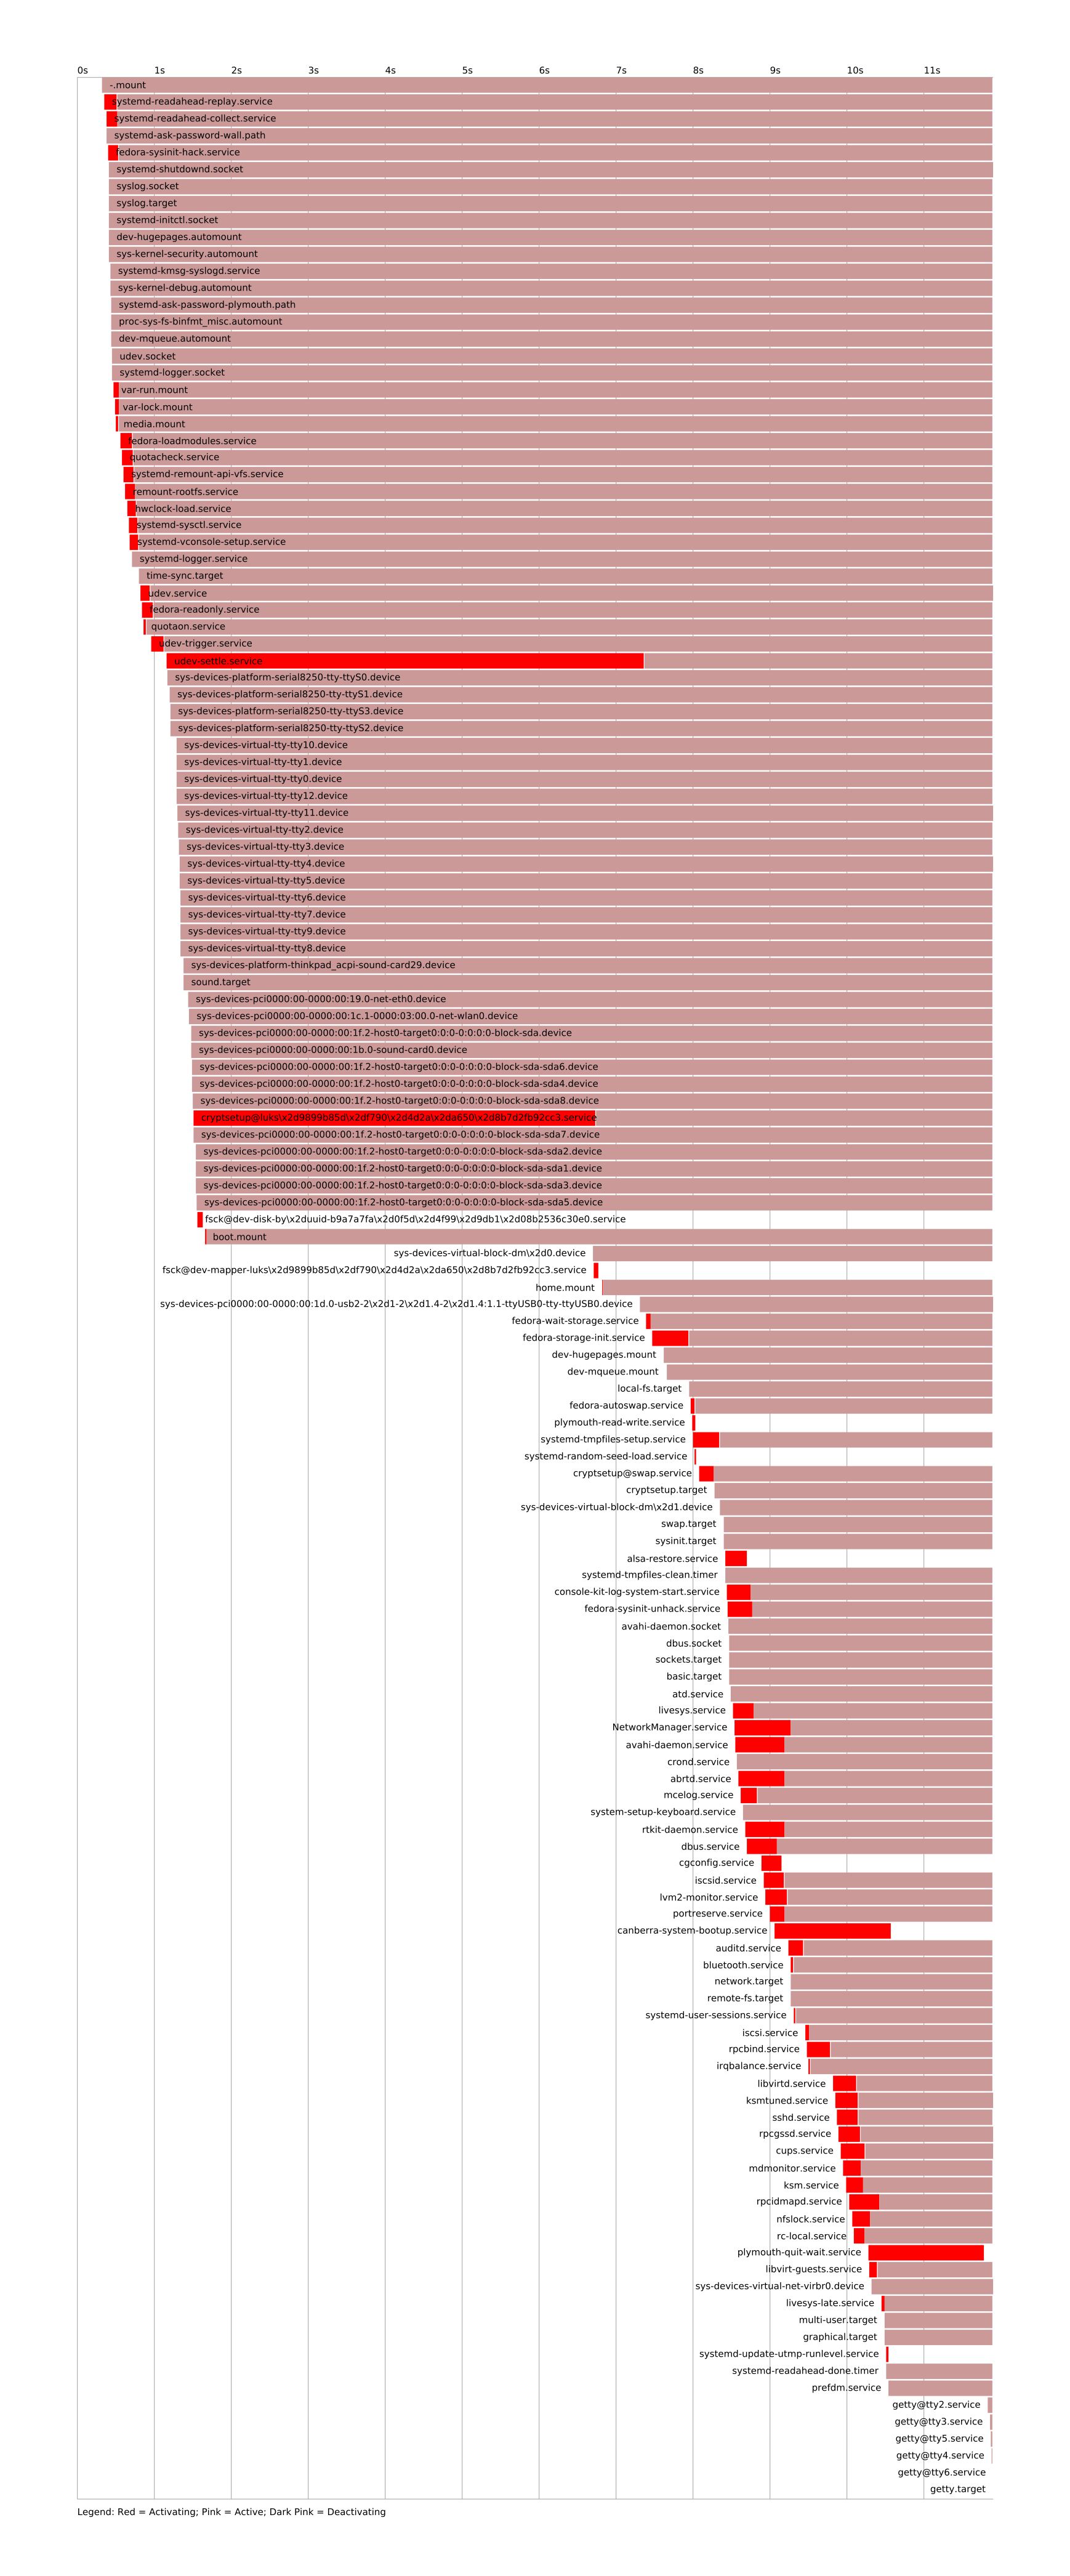
\includegraphics[scale=0.1]{blame.png}
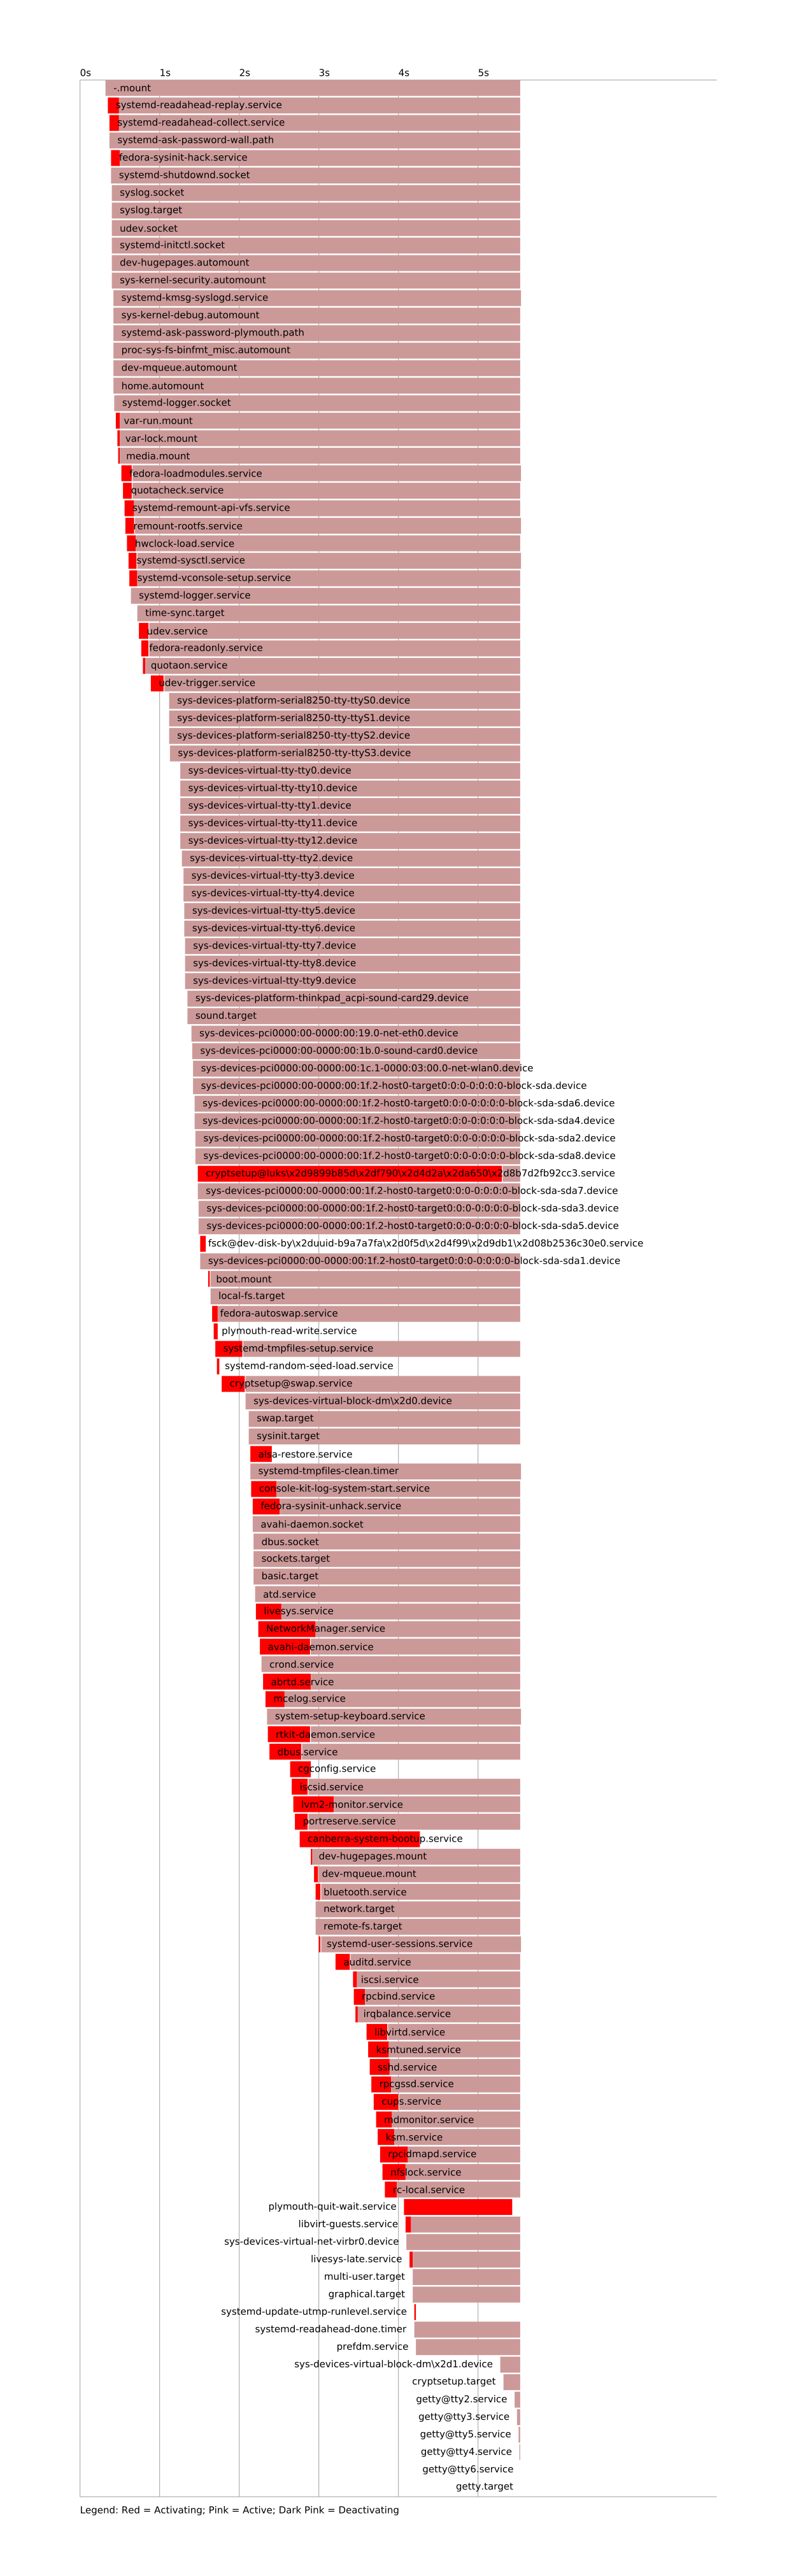
\includegraphics[scale=0.1]{blame2.png}
\\
(For the sake of completeness, here are the two complete outputs of systemd-analyze blame for these two boots: \href{https://0pointer.de/public/blame.txt}{before} and \href{https://0pointer.de/public/blame2.txt}{after}.)
\\
\\
The well-informed reader probably wonders how this relates to \href{https://github.com/mmeeks/bootchart}{Michael Meeks' bootchart}. This plot and bootchart do show similar graphs, that is true. Bootchart is by far the more powerful tool. It plots in all detail what is happening during the boot, how much CPU and IO is used. systemd-analyze plot shows more high-level data: which service took how much time to initialize, and what needed to wait for it. If you use them both together you'll have a wonderful toolset to figure out why your boot is not as fast as it could be.
\\
\\
Now, before you now take these tools and start filing bugs against the worst boot-up time offenders on your system: think twice. These tools give you raw data, don't misread it. As my optimization example above hopefully shows, the blame for the slow bootup was not actually with udev-settle.service, and not with the ModemManager prober run by it either. It is with the subsystem that pulled this service in in the first place. And that's where the problem needs to be fixed. So, file the bugs at the right places. Put the blame where the blame belongs.
\\
\\
As mentioned, these three utilities are available on your Fedora 15 system out-of-the-box.
\\
\\
And here's what to take home from this little blog story:
\begin{itemize}
\item
systemd-analyze is a wonderful tool and systemd comes with profiling built in.
\item
Don't misread the data these tools generate!
\item
With two simple changes you might be able to speed up your system by 7s!
\item
Fix your software if it can't handle dynamic hardware properly!
\item
The Fedora default of installing the OS on an enterprise-level storage managing system might be something to rethink.
\end{itemize}
\section{The New Configuration Files}
One of the formidable new features of systemd is that it comes with a complete set of modular early-boot services that are written in simple, fast, parallelizable and robust C, replacing the shell "novels" the various distributions featured before. Our little Project Zero Shell[1] has been a full success. We currently cover pretty much everything most desktop and embedded distributions should need, plus a big part of the server needs:
\begin{itemize}
\item Checking and mounting of all file systems
\item Updating and enabling quota on all file systems
\item Setting the host name
\item Configuring the loopback network device
\item Loading the SELinux policy and relabelling /run and /dev as necessary on boot
\item Registering additional binary formats in the kernel, such as Java, Mono and WINE binaries
\item Setting the system locale
\item Setting up the console font and keyboard map
\item Creating, removing and cleaning up of temporary and volatile files and directories
\item Applying mount options from /etc/fstab to pre-mounted API VFS
\item Applying sysctl kernel settings
\item Collecting and replaying readahead information
\item Updating utmp boot and shutdown records
\item Loading and saving the random seed
\item Statically loading specific kernel modules
\item Setting up encrypted hard disks and partitions
\item Spawning automatic gettys on serial kernel consoles
\item Maintenance of Plymouth
\item Machine ID maintenance
\item Setting of the UTC distance for the system clock
\end{itemize}
On a standard Fedora 15 install, only a few legacy and storage services still require shell scripts during early boot. If you don't need those, you can easily disable them end enjoy your shell-free boot (like I do every day). The shell-less boot systemd offers you is a unique feature on Linux.
\\
\\
Many of these small components are configured via configuration files in /etc. Some of these are fairly standardized among distributions and hence supporting them in the C implementations was easy and obvious. Examples include: /etc/fstab, /etc/crypttab or /etc/sysctl.conf. However, for others no standardized file or directory existed which forced us to add #ifdef orgies to our sources to deal with the different places the distributions we want to support store these things. All these configuration files have in common that they are dead-simple and there is simply no good reason for distributions to distuingish themselves with them: they all do the very same thing, just a bit differently.
\\
\\
To improve the situation and benefit from the unifying force that systemd is we thus decided to read the per-distribution configuration files only as fallbacks -- and to introduce new configuration files as primary source of configuration wherever applicable. Of course, where possible these standardized configuration files should not be new inventions but rather just standardizations of the best distribution-specific configuration files previously used. Here's a little overview over these new common configuration files systemd supports on all distributions:
\begin{itemize}
\item \href{https://0pointer.de/public/systemd-man/hostname.html}{/etc/hostname}: the host name for the system. One of the most basic and trivial system settings. Nonetheless previously all distributions used different files for this. Fedora used /etc/sysconfig/network, OpenSUSE /etc/HOSTNAME. We chose to standardize on the Debian configuration file /etc/hostname.
\item \href{https://0pointer.de/public/systemd-man/vconsole.conf.html}{/etc/vconsole.conf}: configuration of the default keyboard mapping and console font.
\item \href{https://0pointer.de/public/systemd-man/locale.conf.html}{/etc/locale.conf}: configuration of the system-wide locale.
\item \href{https://0pointer.de/public/systemd-man/modules-load.d.html}{/etc/modules-load.d/*.conf}: a drop-in directory for kernel modules to statically load at boot (for the very few that still need this).
\item \href{https://0pointer.de/public/systemd-man/sysctl.d.html}{/etc/sysctl.d/*.conf}: a drop-in directory for kernel sysctl parameters, extending what you can already do with /etc/sysctl.conf.
\item \href{https://0pointer.de/public/systemd-man/tmpfiles.d.html}{/etc/tmpfiles.d/*.conf}: a drop-in directory for configuration of runtime files that need to be removed/created/cleaned up at boot and during uptime.
\item \href{https://0pointer.de/public/systemd-man/binfmt.d.html}{/etc/binfmt.d/*.conf}: a drop-in directory for registration of additional binary formats for systems like Java, Mono and WINE.
\item \href{https://0pointer.de/public/systemd-man/os-release.html}{/etc/os-release}: a standardization of the various distribution ID files like /etc/fedora-release and similar. Really every distribution introduced their own file here; writing a simple tool that just prints out the name of the local distribution usually means including a database of release files to check. The LSB tried to standardize something like this with the lsb\_release tool, but quite frankly the idea of employing a shell script in this is not the best choice the LSB folks ever made. To rectify this we just decided to generalize this, so that everybody can use the same file here.
\item \href{https://0pointer.de/public/systemd-man/machine-id.html}{/etc/machine-id}: a machine ID file, superseding D-Bus' machine ID file. This file is guaranteed to be existing and valid on a systemd system, covering also stateless boots. By moving this out of the D-Bus logic it is hopefully interesting for a lot of additional uses as a unique and stable machine identifier.
\item \href{https://0pointer.de/public/systemd-man/machine-info.html}{/etc/machine-info}: a new information file encoding meta data about a host, like a pretty host name and an icon name, replacing stuff like /etc/favicon.png and suchlike. This is maintained by \href{https://www.freedesktop.org/wiki/Software/systemd/hostnamed}{systemd-hostnamed}.
\end{itemize}
I is our definite intention to convince you to use these new configuration files in your configuration tools: if your configuration frontend writes these files instead of the old ones, it automatically becomes more portable between Linux distributions, and you are helping standardizing Linux. This makes things simpler to understand and more obvious for users and administrators. Of course, right now, only systemd-based distributions read these files, but that already covers all important distributions in one way or another, \href{https://www.ubuntu.com/}{except for one}. And it's a bit of a chicken-and-egg problem: a standard becomes a standard by being used. In order to gently push everybody to standardize on these files we also want to make clear that sooner or later we plan to drop the fallback support for the old configuration files from systemd. That means adoption of this new scheme can happen slowly and piece by piece. But the final goal of only having one set of configuration files must be clear.
\\
\\
Many of these configuration files are relevant not only for configuration tools but also (and sometimes even primarily) in upstream projects. For example, we invite projects like Mono, Java, or WINE to install a drop-in file in /etc/binfmt.d/ from their upstream build systems. Per-distribution downstream support for binary formats would then no longer be necessary and your platform would work the same on all distributions. Something similar applies to all software which need creation/cleaning of certain runtime files and directories at boot, for example beneath the /run hierarchy (i.e. /var/run as \href{https://lwn.net/Articles/436012/}{it used to be known}). These projects should just drop in configuration files in /etc/tmpfiles.d, also from the upstream build systems. This also helps speeding up the boot process, as separate per-project SysV shell scripts which implement trivial things like registering a binary format or removing/creating temporary/volatile files at boot are no longer necessary. Or another example, where upstream support would be fantastic: projects like X11 could probably benefit from reading the default keyboard mapping for its displays from /etc/vconsole.conf.
\\
\\
Of course, I have no doubt that not everybody is happy with our choice of names (and formats) for these configuration files. In the end we had to pick something, and from all the choices these appeared to be the most convincing. The file formats are as simple as they can be, and usually easily written and read even from shell scripts. That said, /etc/bikeshed.conf could of course also have been a fantastic configuration file name!
\\
\\
\textbf{So, help us standardizing Linux! Use the new configuration files! Adopt them upstream, adopt them downstream, adopt them all across the distributions!}
\\
\\
Oh, and in case you are wondering: yes, all of these files were discussed in one way or another with various folks from the various distributions. And there has even been some push towards supporting some of these files even outside of systemd systems.
\section{On /etc/sysconfig and /etc/default}
So, here's a bit of an opinion piece on the /etc/sysconfig/ and /etc/default directories that exist on the various distributions in one form or another, and why I believe their use should be faded out. Like everything I say on this blog what follows is just my personal opinion, and not the gospel and has nothing to do with the position of the Fedora project or my employer. The topic of /etc/sysconfig has been coming up in discussions over and over again. I hope with this blog story I can explain a bit what we as systemd upstream think about these files.
\\
\\
A few lines about the historical context: I wasn't around when /etc/sysconfig was introduced -- suffice to say it has been around on Red Hat and SUSE distributions since a long long time. Eventually /etc/default was introduced on Debian with very similar semantics. Many other distributions know a directory with similar semantics too, most of them call it either one or the other way. In fact, even other Unix-OSes sported a directory like this. (Such as SCO. If you are interested in the details, I am sure a Unix greybeard of your trust can fill in what I am leaving vague here.) So, even though a directory like this has been known widely on Linuxes and Unixes, it never has been standardized, neither in POSIX nor in LSB/FHS. These directories very much are something where distributions distuingish themselves from each other.
\\
\\
The semantics of /etc/default and /etc/sysconfig are very losely defined only. What almost all files stored in these directories have in common though is that they are sourcable shell scripts which primarily consist of environment variable assignments. Most of the files in these directories are sourced by the SysV init scripts of the same name. The Debian Policy Manual (9.3.2) and the Fedora Packaging Guidelines suggest this use of the directories, however both distributions also have files in them that do not follow this scheme, i.e. that do not have a matching SysV init script -- or not even are shell scripts at all.
\\
\\
Why have these files been introduced? On SysV systems services are started via init scripts in /etc/rc.d/init.d (or a similar directory). /etc/ is (these days) considered the place where system configuration is stored. Originally these init scripts were subject to customization by the administrator. But as they grew and become complex most distributions no longer considered them true configuration files, but more just a special kind of programs. To make customization easy and guarantee a safe upgrade path the customizable bits hence have been moved to separate configuration files, which the init scripts then source.
\\
\\
Let's have a quick look what kind of configuration you can do with these files. Here's a short incomprehensive list of various things that can be configured via environment settings in these source files I found browsing through the directories on a Fedora and a Debian machine:
\begin{itemize}
\item Additional command line parameters for the daemon binaries
\item Locale settings for a daemon
\item Shutdown time-out for a daemon
\item Shutdown mode for a daemon
\item System configuration like system locale, time zone information, console keyboard
\item Redundant system configuration, like whether the RTC is in local timezone
\item Firewall configuration data, not in shell format (!)
\item CPU affinity for a daemon
\item Settings unrelated to boot, for example including information how to install a new kernel package, how to configure nspluginwrap or whether to do library prelinking
\item Whether a specific service should be started or not
\item Networking configuration
\item Which kernel modules to statically load
\item Whether to halt or power-off on shutdown
\item Access modes for device nodes (!)
\item A description string for the SysV service (!)
\item The user/group ID, umask to run specific daemons as
\item Resource limits to set for a specific daemon
\item OOM adjustment to set for a specific daemon
\end{itemize}
Now, let's go where the beef is: what's wrong with /etc/sysconfig (resp. /etc/default)? Why might it make sense to fade out use of these files in a systemd world?
\begin{itemize}
\item For the majority of these files the reason for having them simply does not exist anymore: systemd unit files are not programs like SysV init scripts were. Unit files are simple, declarative descriptions, that usually do not consist of more than 6 lines or so. They can easily be generated, parsed without a Bourne interpreter and understood by the reader. Also, they are very easy to modify: just copy them from /lib/systemd/system to /etc/systemd/system and edit them there, where they will not be modified by the package manager. The need to separate code and configuration that was the original reason to introduce these files does not exist anymore, as systemd unit files do not include code. These files hence now are a solution looking for a problem that no longer exists.
\item They are inherently distribution-specific. With systemd we hope to encourage standardization between distributions. Part of this is that we want that unit files are supplied with upstream, and not just added by the packager -- how it has usually been done in the SysV world. Since the location of the directory and the available variables in the files is very different on each distribution, supporting /etc/sysconfig files in upstream unit files is not feasible. Configuration stored in these files works against de-balkanization of the Linux platform.
\item Many settings are fully redundant in a systemd world. For example, various services support configuration of the process credentials like the user/group ID, resource limits, CPU affinity or the OOM adjustment settings. However, these settings are supported only by some SysV init scripts, and often have different names if supported in multiple of them. OTOH in systemd, all these settings are available equally and uniformly for all services, with the same configuration option in unit files.
\item Unit files know a large number of easy-to-use process context settings, that are more comprehensive than what most /etc/sysconfig files offer.
\item A number of these settings are entirely questionnabe. For example, the aforementiond configuration option for the user/group ID a service runs as is primarily something the distributor has to take care of. There is little to win for administrators to change these settings, and only the distributor has the broad overview to make sure that UID/GID and name collisions do not happen.
\item The file format is not ideal. Since the files are usually sourced as shell scripts, parse errors are very hard to decypher and are not logged along the other configuration problems of the services. Generally, unknown variable assignments simply have no effect but this is not warned about. This makes these files harder to debug than necessary.
\item Configuration files sources from shell scripts are subject to the execution parameters of the interpreter, and it has many: settings like IFS or LANG tend to modify drastically how shell scripts are parsed and understood. This makes them fragile.
\item Interpretation of these files is slow, since it requires spawning of a shell, which adds at least one process for each service to be spawned at boot.
\item Often, files in /etc/sysconfig are used to "fake" configuration files for daemons which do not support configuration files natively. This is done by glueing together command line arguments from these variable assignments that are then passed to the daemon. In general proper, native configuration files in these daemons are the much prettier solution however. Command line options like "-k", "-a" or "-f" are not self-explanatory and have a very cryptic syntax. Moreover the same switches in many daemons have (due to the limited vocabulary) often very much contradicting effects. (On one daemon -f might cause the daemon to daemonize, while on another one this option turns exactly this behaviour off.) Command lines generally cannot include sensible comments which most configuration files however can.
\item A number of configuration settings in /etc/sysconfig are entirely redundant: for example, on many distributions it can be controlled via /etc/sysconfig files whether the RTC is in UTC or local time. Such an option already exists however in the 3rd line of the /etc/adjtime (which is known on all distributions). Adding a second, redundant, distribution-specific option overriding this is hence needless and complicates things for no benefit.
\item Many of the configuration settings in /etc/sysconfig allow disabling services. By this they basically become a second level of enabling/disabling over what the init system already offers: when a service is enabled with systemctl enable or chkconfig on these settings override this, and turn the daemon of even though the init system was configured to start it. This of course is very confusing to the user/administrator, and brings virtually no benefit.
\item For options like the configuration of static kernel modules to load: there are nowadays usually much better ways to load kernel modules at boot. For example, most modules may now be autoloaded by udev when the right hardware is found. This goes very far, and even includes ACPI and other high-level technologies. One of the very few exceptions where we currently do not do kernel module autoloading is CPU feature and model based autoloading which however will be supported soon too. And even if your specific module cannot be auto-loaded there's usually a better way to statically load it, for example by sticking it in /etc/load-modules.d so that the administrator can check a standardized place for all statically loaded modules.
\item Last but not least, /etc already is intended to be the place for system configuration ("Host-specific system configuration" according to FHS). A subdirectory beneath it called sysconfig to place system configuration in is hence entirely redundant, already on the language level.
\end{itemize}
What to use instead? Here are a few recommendations of what to do with these files in the long run in a systemd world:
\begin{itemize}
\item Just drop them without replacement. If they are fully redundant (like the local/UTC RTC setting) this is should be a relatively easy way out (well, ignoring the need for compatibility). If systemd natively supports an equivalent option in the unit files there is no need to duplicate these settings in sysconfig files. For a list of execution options you may set for a service check out the respective man pages: systemd.exec(5) and systemd.service(5). If your setting simply adds another layer where a service can be disabled, remove it to keep things simple. There's no need to have multiple ways to disable a service.
\item Find a better place for them. For configuration of the system locale or system timezone we hope to gently push distributions into the right direction, for more details see previous episode of this series.
\item Turn these settings into native settings of the daemon. If necessary add support for reading native configuration files to the daemon. Thankfully, most of the stuff we run on Linux is Free Software, so this can relatively easily be done.
\end{itemize}
Of course, there's one very good reason for supporting these files for a bit longer: compatibility for upgrades. But that's is really the only one I could come up with. It's reason enough to keep compatibility for a while, but I think it is a good idea to phase out usage of these files at least in new packages.
\\
\\
If compatibility is important, then systemd will still allow you to read these configuration files even if you otherwise use native systemd unit files. If your sysconfig file only knows simple options EnvironmentFile=-/etc/sysconfig/foobar (See systemd.exec(5) for more information about this option.) may be used to import the settings into the environment and use them to put together command lines. If you need a programming language to make sense of these settings, then use a programming language like shell. For example, place an short shell script in /usr/lib/<your package>/ which reads these files for compatibility, and then exec's the actual daemon binary. Then spawn this script instead of the actual daemon binary with ExecStart= in the unit file.
\section{Instantiated Services}
Most services on Linux/Unix are singleton services: there's usually only one instance of Syslog, Postfix, or Apache running on a specific system at the same time. On the other hand some select services may run in multiple instances on the same host. For example, an Internet service like the Dovecot IMAP service could run in multiple instances on different IP ports or different local IP addresses. A more common example that exists on all installations is getty, the mini service that runs once for each TTY and presents a login prompt on it. On most systems this service is instantiated once for each of the first six virtual consoles tty1 to tty6. On some servers depending on administrator configuration or boot-time parameters an additional getty is instantiated for a serial or virtualizer console. Another common instantiated service in the systemd world is fsck, the file system checker that is instantiated once for each block device that needs to be checked. Finally, in systemd socket activated per-connection services (think classic inetd!) are also implemented via instantiated services: a new instance is created for each incoming connection. In this installment I hope to explain a bit how systemd implements instantiated services and how to take advantage of them as an administrator.
\\
\\
If you followed the previous episodes of this series you are probably aware that services in systemd are named according to the pattern foobar.service, where foobar is an identification string for the service, and .service simply a fixed suffix that is identical for all service units. The definition files for these services are searched for in /etc/systemd/system and /lib/systemd/system (and possibly other directories) under this name. For instantiated services this pattern is extended a bit: the service name becomes foobar@quux.service where foobar is the common service identifier, and quux the instance identifier. Example: serial-getty@ttyS2.service is the serial getty service instantiated for ttyS2.
\\
\\
Service instances can be created dynamically as needed. Without further configuration you may easily start a new getty on a serial port simply by invoking a systemctl start command for the new instance:
\begin{lstlisting}
# systemctl start serial-getty@ttyUSB0.service
\end{lstlisting}
If a command like the above is run systemd will first look for a unit configuration file by the exact name you requested. If this service file is not found (and usually it isn't if you use instantiated services like this) then the instance id is removed from the name and a unit configuration file by the resulting template name searched. In other words, in the above example, if the precise serial-getty@ttyUSB0.service unit file cannot be found, serial-getty@.service is loaded instead. This unit template file will hence be common for all instances of this service. For the serial getty we ship a template unit file in systemd (/lib/systemd/system/serial-getty@.service) that looks something like this:
\begin{lstlisting}
[Unit]
Description=Serial Getty on %I
BindTo=dev-%i.device
After=dev-%i.device systemd-user-sessions.service

[Service]
ExecStart=-/sbin/agetty -s %I 115200,38400,9600
Restart=always
RestartSec=0
\end{lstlisting}
(Note that the unit template file we actually ship along with systemd for the serial gettys is a bit longer. If you are interested, have a look at the actual file which includes additional directives for compatibility with SysV, to clear the screen and remove previous users from the TTY device. To keep things simple I have shortened the unit file to the relevant lines here.)
\\
\\
This file looks mostly like any other unit file, with one distinction: the specifiers \%I and \%i are used at multiple locations. At unit load time \%I and \%i are replaced by systemd with the instance identifier of the service. In our example above, if a service is instantiated as serial-getty@ttyUSB0.service the specifiers \%I and \%i will be replaced by ttyUSB0. If you introspect the instanciated unit with systemctl status serial-getty@ttyUSB0.service you will see these replacements having taken place:
\begin{lstlisting}
$ systemctl status serial-getty@ttyUSB0.service
serial-getty@ttyUSB0.service - Getty on ttyUSB0
      Loaded: loaded (/lib/systemd/system/serial-getty@.service; static)
      Active: active (running) since Mon, 26 Sep 2011 04:20:44 +0200; 2s ago
    Main PID: 5443 (agetty)
      CGroup: name=systemd:/system/getty@.service/ttyUSB0
          └ 5443 /sbin/agetty -s ttyUSB0 115200,38400,9600
\end{lstlisting}
And that is already the core idea of instantiated services in systemd. As you can see systemd provides a very simple templating system, which can be used to dynamically instantiate services as needed. To make effective use of this, a few more notes:
\\
You may instantiate these services on-the-fly in .wants/ symbolic links in the file system. For example, to make sure the serial getty on ttyUSB0 is started automatically at every boot, create a symlink like this:
\begin{lstlisting}
# ln -s /lib/systemd/system/serial-getty@.service \
    /etc/systemd/system/getty.target.wants/serial-getty@ttyUSB0.service
\end{lstlisting}
systemd will instantiate the symlinked unit file with the instance name specified in the symlink name.
\\
\\
You cannot instantiate a unit template without specifying an instance identifier. In other words systemctl start serial-getty@.service will necessarily fail since the instance name was left unspecified.
\\
\\
Sometimes it is useful to opt-out of the generic template for one specific instance. For these cases make use of the fact that systemd always searches first for the full instance file name before falling back to the template file name: make sure to place a unit file under the fully instantiated name in /etc/systemd/system and it will override the generic templated version for this specific instance.
\\
\\
The unit file shown above uses \%i at some places and \%I at others. You may wonder what the difference between these specifiers are. \%i is replaced by the exact characters of the instance identifier. For \%I on the other hand the instance identifier is first passed through a simple unescaping algorithm. In the case of a simple instance identifier like ttyUSB0 there is no effective difference. However, if the device name includes one or more slashes ("/") this cannot be part of a unit name (or Unix file name). Before such a device name can be used as instance identifier it needs to be escaped so that "/" becomes "-" and most other special characters (including "-") are replaced by "\\xAB" where AB is the ASCII code of the character in hexadecimal notation[1]. Example: to refer to a USB serial port by its bus path we want to use a port name like serial/by-path/pci-0000:00:1d.0-usb-0:1.4:1.1-port0. The escaped version of this name is serial-by\\x2dpath-pci\\x2d0000:00:1d.0\\x2dusb\\x2d0:1.4:1.1\\x2dport0. \%I will then refer to former, \%i to the latter. Effectively this means \%i is useful wherever it is necessary to refer to other units, for example to express additional dependencies. On the other hand \%I is useful for usage in command lines, or inclusion in pretty description strings. Let's check how this looks with the above unit file:
\begin{lstlisting}
# systemctl start \
'serial-getty@serial-by\x2dpath-pci\x2d0000:00:1d.0\x2dusb
\x2d0:1.4:1.1\x2dport0.service'
# systemctl status \
'serial-getty@serial-by\x2dpath-pci\x2d0000:00:1d.0\x2dusb
\x2d0:1.4:1.1\x2dport0.service'
serial-getty@serial-by\x2dpath-pci\x2d0000:00:1d.0\x2dusb
\x2d0:1.4:1.1\x2dport0.service \
- Serial Getty on serial/by-path/pci-0000:00:1d.0-usb-0:1.4:1.1-port0
  Loaded: loaded (/lib/systemd/system/serial-getty@.service; static)
  Active: active (running) since Mon, 26 Sep 2011 05:08:52 +0200; 1s ago
  Main PID: 5788 (agetty)
  CGroup: 
name=systemd:/system/serial-getty@.service/serial-by
\x2dpath-pci\x2d0000:00:1d.0\x2dusb\x2d0:1.4:1.1\x2dport0
    └ 5788 /sbin/agetty -s serial/by-path/pci-0000:00:
1d.0-usb-0:1.4:1.1-port0 115200 38400 9600
\end{lstlisting}
As we can see the while the instance identifier is the escaped string the command line and the description string actually use the unescaped version, as expected.
\\
\\
(Side note: there are more specifiers available than just \%i and \%I, and many of them are actually available in all unit files, not just templates for service instances. For more details see the man page which includes a full list and terse explanations.)
\\
\\
And at this point this shall be all for now. Stay tuned for a follow-up article on how instantiated services are used for inetd-style socket activation.
\section{Converting inetd Services}
In a previous episode of this series I covered how to convert a SysV init script to a systemd unit file. In this story I hope to explain how to convert inetd services into systemd units.
\\
\\
Let's start with a bit of background. inetd has a long tradition as one of the classic Unix services. As a superserver it listens on an Internet socket on behalf of another service and then activate that service on an incoming connection, thus implementing an on-demand socket activation system. This allowed Unix machines with limited resources to provide a large variety of services, without the need to run processes and invest resources for all of them all of the time. Over the years a number of independent implementations of inetd have been shipped on Linux distributions. The most prominent being the ones based on BSD inetd and xinetd. While inetd used to be installed on most distributions by default, it nowadays is used only for very few selected services and the common services are all run unconditionally at boot, primarily for (perceived) performance reasons.
\\
\\
One of the core feature of systemd (and Apple's launchd for the matter) is socket activation, a scheme pioneered by inetd, however back then with a different focus. Systemd-style socket activation focusses on local sockets (AF\_UNIX), not so much Internet sockets (AF\_INET), even though both are supported. And more importantly even, socket activation in systemd is not primarily about the on-demand aspect that was key in inetd, but more on increasing parallelization (socket activation allows starting clients and servers of the socket at the same time), simplicity (since the need to configure explicit dependencies between services is removed) and robustness (since services can be restarted or may crash without loss of connectivity of the socket). However, systemd can also activate services on-demand when connections are incoming, if configured that way.
\\
\\
Socket activation of any kind requires support in the services themselves. systemd provides a very simple interface that services may implement to provide socket activation, built around sd\_listen\_fds(). As such it is already a very minimal, simple scheme. However, the traditional inetd interface is even simpler. It allows passing only a single socket to the activated service: the socket fd is simply duplicated to STDIN and STDOUT of the process spawned, and that's already it. In order to provide compatibility systemd optionally offers the same interface to processes, thus taking advantage of the many services that already support inetd-style socket activation, but not yet systemd's native activation.
\\
\\
Before we continue with a concrete example, let's have a look at three different schemes to make use of socket activation:
\begin{enumerate}
\item Socket activation for parallelization, simplicity, robustness: sockets are bound during early boot and a singleton service instance to serve all client requests is immediately started at boot. This is useful for all services that are very likely used frequently and continously, and hence starting them early and in parallel with the rest of the system is advisable. Examples: D-Bus, Syslog.
\item On-demand socket activation for singleton services: sockets are bound during early boot and a singleton service instance is executed on incoming traffic. This is useful for services that are seldom used, where it is advisable to save the resources and time at boot and delay activation until they are actually needed. Example: CUPS.
\item On-demand socket activation for per-connection service instances: sockets are bound during early boot and for each incoming connection a new service instance is instantiated and the connection socket (and not the listening one) is passed to it. This is useful for services that are seldom used, and where performance is not critical, i.e. where the cost of spawning a new service process for each incoming connection is limited. Example: SSH.
\end{enumerate}
The three schemes provide different performance characteristics. After the service finishes starting up the performance provided by the first two schemes is identical to a stand-alone service (i.e. one that is started without a super-server, without socket activation), since the listening socket is passed to the actual service, and code paths from then on are identical to those of a stand-alone service and all connections are processes exactly the same way as they are in a stand-alone service. On the other hand, performance of the third scheme is usually not as good: since for each connection a new service needs to be started the resource cost is much higher. However, it also has a number of advantages: for example client connections are better isolated and it is easier to develop services activated this way.
\\
\\
For systemd primarily the first scheme is in focus, however the other two schemes are supported as well. (In fact, the blog story I covered the necessary code changes for systemd-style socket activation in was about a service of the second type, i.e. CUPS). inetd primarily focusses on the third scheme, however the second scheme is supported too. (The first one isn't. Presumably due the focus on the third scheme inetd got its -- a bit unfair -- reputation for being "slow".)
\\
\\
So much about the background, let's cut to the beef now and show an inetd service can be integrated into systemd's socket activation. We'll focus on SSH, a very common service that is widely installed and used but on the vast majority of machines probably not started more often than 1/h in average (and usually even much less). SSH has supported inetd-style activation since a long time, following the third scheme mentioned above. Since it is started only every now and then and only with a limited number of connections at the same time it is a very good candidate for this scheme as the extra resource cost is negligble: if made socket-activatable SSH is basically free as long as nobody uses it. And as soon as somebody logs in via SSH it will be started and the moment he or she disconnects all its resources are freed again. Let's find out how to make SSH socket-activatable in systemd taking advantage of the provided inetd compatibility!
\\
\\
Here's the configuration line used to hook up SSH with classic inetd:
\begin{lstlisting}
ssh stream tcp nowait root /usr/sbin/sshd sshd -i
\end{lstlisting}
And the same as xinetd configuration fragment:
\begin{lstlisting}
service ssh {
        socket_type = stream
        protocol = tcp
        wait = no
        user = root
        server = /usr/sbin/sshd
        server_args = -i
}
\end{lstlisting}
Most of this should be fairly easy to understand, as these two fragments express very much the same information. The non-obvious parts: the port number (22) is not configured in inetd configuration, but indirectly via the service database in /etc/services: the service name is used as lookup key in that database and translated to a port number. This indirection via /etc/services has been part of Unix tradition though has been getting more and more out of fashion, and the newer xinetd hence optionally allows configuration with explicit port numbers. The most interesting setting here is the not very intuitively named nowait (resp. wait=no) option. It configures whether a service is of the second (wait) resp. third (nowait) scheme mentioned above. Finally the -i switch is used to enabled inetd mode in SSH.
\\
\\
The systemd translation of these configuration fragments are the following two units. First: sshd.socket is a unit encapsulating information about a socket to listen on:
\begin{lstlisting}
[Unit]
Description=SSH Socket for Per-Connection Servers

[Socket]
ListenStream=22
Accept=yes

[Install]
WantedBy=sockets.target
\end{lstlisting}
Most of this should be self-explanatory. A few notes: Accept=yes corresponds to nowait. It's hopefully better named, referring to the fact that for nowait the superserver calls accept() on the listening socket, where for wait this is the job of the executed service process. WantedBy=sockets.target is used to ensure that when enabled this unit is activated at boot at the right time.
\\
\\
And here's the matching service file sshd@.service:
\begin{lstlisting}
[Unit]
Description=SSH Per-Connection Server

[Service]
ExecStart=-/usr/sbin/sshd -i
StandardInput=socket
\end{lstlisting}
This too should be mostly self-explanatory. Interesting is StandardInput=socket, the option that enables inetd compatibility for this service. StandardInput= may be used to configure what STDIN of the service should be connected for this service (see the man page for details). By setting it to socket we make sure to pass the connection socket here, as expected in the simple inetd interface. Note that we do not need to explicitly configure StandardOutput= here, since by default the setting from StandardInput= is inherited if nothing else is configured. Important is the "-" in front of the binary name. This ensures that the exit status of the per-connection sshd process is forgotten by systemd. Normally, systemd will store the exit status of a all service instances that die abnormally. SSH will sometimes die abnormally with an exit code of 1 or similar, and we want to make sure that this doesn't cause systemd to keep around information for numerous previous connections that died this way (until this information is forgotten with systemctl reset-failed).
\\
\\
sshd@.service is an instantiated service, as described in the preceeding installment of this series. For each incoming connection systemd will instantiate a new instance of sshd@.service, with the instance identifier named after the connection credentials.
\\
\\
You may wonder why in systemd configuration of an inetd service requires two unit files instead of one. The reason for this is that to simplify things we want to make sure that the relation between live units and unit files is obvious, while at the same time we can order the socket unit and the service units independently in the dependency graph and control the units as independently as possible. (Think: this allows you to shutdown the socket independently from the instances, and each instance individually.)
\\
\\
Now, let's see how this works in real life. If we drop these files into /etc/systemd/system we are ready to enable the socket and start it:
\begin{lstlisting}
# systemctl enable sshd.socket
ln -s '/etc/systemd/system/sshd.socket' \
  '/etc/systemd/system/sockets.target.wants/sshd.socket'
# systemctl start sshd.socket
# systemctl status sshd.socket
sshd.socket - SSH Socket for Per-Connection Servers
      Loaded: loaded (/etc/systemd/system/sshd.socket; enabled)
      Active: active (listening) since Mon, 26 Sep 2011 20:24:31 +0200; 14s ago
    Accepted: 0; Connected: 0
      CGroup: name=systemd:/system/sshd.socket
\end{lstlisting}
This shows that the socket is listening, and so far no connections have been made (Accepted: will show you how many connections have been made in total since the socket was started, Connected: how many connections are currently active.)
\\
\\
Now, let's connect to this from two different hosts, and see which services are now active:
\begin{lstlisting}
$ systemctl --full | grep ssh
sshd@172.31.0.52:22-172.31.0.4:47779.service  loaded active running       
sshd@172.31.0.52:22-172.31.0.54:52985.service loaded active running       
sshd.socket                                   loaded active listening     
\end{lstlisting}
As expected, there are now two service instances running, for the two connections, and they are named after the source and destination address of the TCP connection as well as the port numbers. (For AF\_UNIX sockets the instance identifier will carry the PID and UID of the connecting client.) This allows us to invidiually introspect or kill specific sshd instances, in case you want to terminate the session of a specific client:
\begin{lstlisting}
# systemctl kill sshd@172.31.0.52:22-172.31.0.4:47779.service
\end{lstlisting}
And that's probably already most of what you need to know for hooking up inetd services with systemd and how to use them afterwards.
\\
\\
In the case of SSH it is probably a good suggestion for most distributions in order to save resources to default to this kind of inetd-style socket activation, but provide a stand-alone unit file to sshd as well which can be enabled optionally. I'll soon file a wishlist bug about this against our SSH package in Fedora.
\\
\\
A few final notes on how xinetd and systemd compare feature-wise, and whether xinetd is fully obsoleted by systemd. The short answer here is that systemd does not provide the full xinetd feature set and that is does not fully obsolete xinetd. The longer answer is a bit more complex: if you look at the multitude of options xinetd provides you'll notice that systemd does not compare. For example, systemd does not come with built-in echo, time, daytime or discard servers, and never will include those. TCPMUX is not supported, and neither are RPC services. However, you will also find that most of these are either irrelevant on today's Internet or became other way out-of-fashion. The vast majority of inetd services do not directly take advantage of these additional features. In fact, none of the xinetd services shipped on Fedora make use of these options. That said, there are a couple of useful features that systemd does not support, for example IP ACL management. However, most administrators will probably agree that firewalls are the better solution for these kinds of problems and on top of that, systemd supports ACL management via tcpwrap for those who indulge in retro technologies like this. On the other hand systemd also provides numerous features xinetd does not provide, starting with the individual control of instances shown above, or the more expressive configurability of the execution context for the instances. I believe that what systemd provides is quite comprehensive, comes with little legacy cruft but should provide you with everything you need. And if there's something systemd does not cover, xinetd will always be there to fill the void as you can easily run it in conjunction with systemd. For the majority of uses systemd should cover what is necessary, and allows you cut down on the required components to build your system from. In a way, systemd brings back the functionality of classic Unix inetd and turns it again into a center piece of a Linux system.
\section{references}
\nocite{*}
\bibliography{references}
\bibliographystyle{plain}
\end{document}
